\documentclass[letter,10pt]{article}
\usepackage{amsfonts}
\usepackage{amsmath}
\usepackage[margin=1.0in]{geometry}
\usepackage{fancyhdr}
\usepackage{hyperref}
\usepackage{multicol}
\usepackage{textcomp}
\usepackage{graphicx}
 %
\setlength{\columnsep}{0.5cm}
\pagestyle{fancy}
\fancyhf{}
\lhead{
	CSE 847: Machine Learning---Project Proposal \\
	Langford, Lingg, and Lucero
}
\rhead{February 17, 2017}
\cfoot{\thepage}
\begin{document}
	\title{
		CSE 847: Machine Learning---Project Proposal \\
		\textbf{An Exploration and Implementation of Automated Valuation Models to Learn and Predict the Value of Real Estate}
	}
	\author{
		\begin{tabular}{ccc}
			Mick Langford & Mike Lingg  & Jordi Lucero \\
			langfo37@msu.edu & linggmic@egr.msu.edu & luceroj2@msu.edu
		\end{tabular}
	}
	\date{February 17, 2017}
	\maketitle
	\begin{multicols}{2}
		\section{Problem Description}
		Automated Valuation Models (AVM) have become increasingly popular as the real estate market has embraced the World Wide Web as a source of accurate, up to the minute data.\textsuperscript{\cite{kaggleblog}} Banks have also shown great interest in using AVMs to help mitigate fraud by human appraisal.\textsuperscript{\cite{scotsman}} Our goal is to explore various machine learning techniques to implement an AVM and predict the true value of a house based on features commonly found on real estate listings.  Our data will be drawn from the Nashville, TN housing market, using a dataset posted on Kaggle\textsuperscript{\cite{kaggledata}}.
		\par
		We will begin by exploring linear regression models that take into account physical attributes of each house and location. Further work will be performed exploring nonlinear models, such as deep learning with neural networks and decision trees, which can be compared and contrasted. Additional work may be performed to explore missing feature estimation.
		\section{Related Work}
		An obvious and popular example is Zillow's proprietary Zestimate\textsuperscript{\textregistered}. Zillow uses a closed source AVM that takes into account special features of the home, location, and market conditions. Zillow admits to using features such as physical attributes, tax assessments, and prior transactions. Zillow claims to have data on 110 million homes and estimates on approximately 100 million homes.\textsuperscript{\cite{zillow}}
		\par
		Relevant papers include the doctoral dissertation of Lowrance which explores and compares various linear models on housing data for the Los Angeles County.\textsuperscript{\cite{lowrance}} Park and Bae explore machine learning algorithms such as C4.5, RIPPER, Naive Bayesian, and AdaBoost.\textsuperscript{\cite{park}} Bin performed a study that estimates a hedonic price function using a semi-parametric regression.\textsuperscript{\cite{bin}} This may be particularly useful for real estate listings that are incomplete or for data that is entered erroneously. Bourassa et al. consider the spatial dependence of house prices, which is intuitively an important factor.\textsuperscript{\cite{bourassa1}\cite{bourassa2}} Kauko et al. research neural network models to help investigate segmentation in the housing market of Helsinki, Finland.\textsuperscript{\cite{kauko}} Azadeh et al. present an algorithm based on fuzzy linear regression and a fuzzy cognitive map to handle uncertainty in the housing market and improve the analysis of housing price fluctuations.\textsuperscript{\cite{azadeh}} Fan et al. introduce a decision tree approach for modeling and predicting house prices.\textsuperscript{\cite{fan}}
		\section{Project Milestones}
		Figure \ref{fig:ganttchart} below shows our project milestones and timeline to completing them. The team's first milestone after the proposal is to design a Linear Regression Model for our Nashville housing dataset. We will then explore the uses of alternative models for our dataset, such as Deep Learning and Decision Trees, and compare them to decide which may yield the most useful results. The previously stated milestones the team expects to have done when the Intermediate Report is completed. After the Intermediate Report is complete, we will implement the models that were decided upon in the previous milestones. From these models, we will gather predictions and anaylze them. The last milestone will be to complete the Final Report with our results. 
		\par

\begin{figure*}[t]
    \centering
    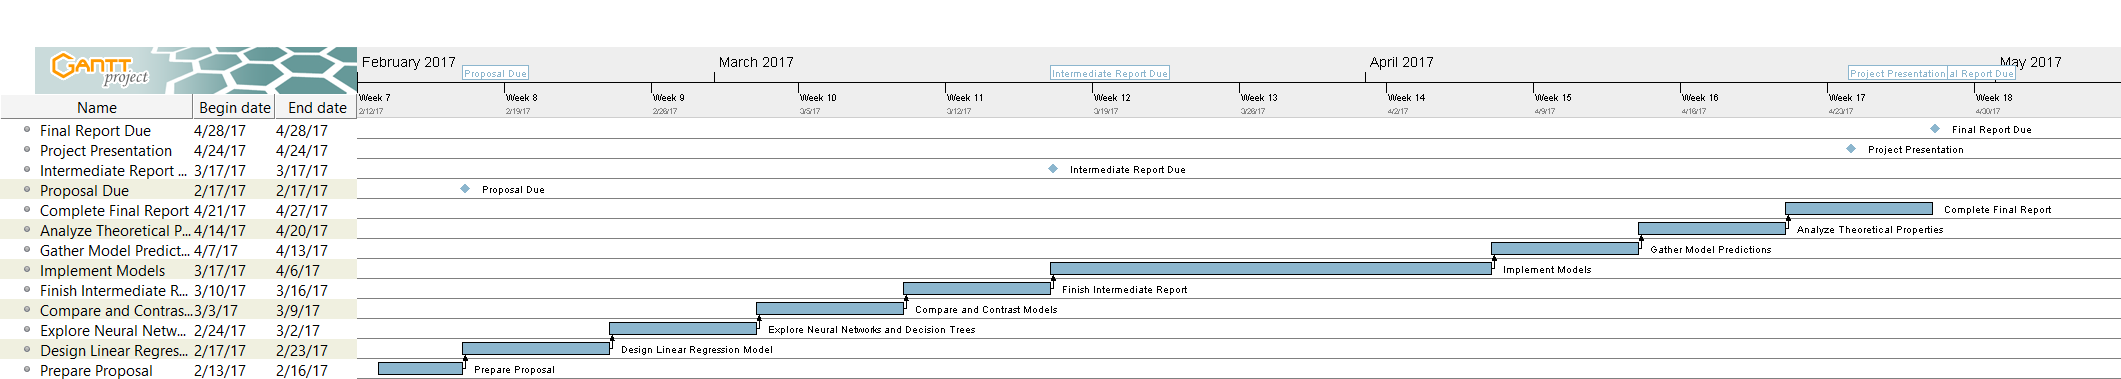
\includegraphics[width=\textwidth]{Schedule/ProjectSchedule.png}
    \caption{Gantt Chart showing  our project milestones and expected completion dates.}
    \label{fig:ganttchart}
\end{figure*}

		\begin{thebibliography}{9}
			\bibitem{kaggledata}
			\textit{Nashville Housing Data: Home value data for the booming Nashville Market}
			Retrieved from \\ \small{\url{https://www.kaggle.com/tmthyjames/nashville-housing-data/}}
			
			\bibitem{kaggleblog}
			\textit{Data-driven property valuations: the real deal?}
			Retrieved from \\ \small{\url{http://blog.kaggle.com/2010/06/21/data-inc-are-avms-soothsayers-or-the-real-deal/}}
			
			\bibitem{scotsman}
			Schroeder, Steve.
			\textit{Fighting Fraud: A combination of collateral assessment and AVMs can maximize mortgage-fraud management}
			Retrieved from \\ \small{\url{http://www.scotsmanguide.com/Residential/Articles/2005/10/Fighting-Fraud/}}
			
			\bibitem{zillow}
			\textit{What is a Zestimate? Zillow's Home Value Forecast.}
			Retrieved from \\
			\small{\url{http://www.zillow.com/zestimate/}}
			
			\bibitem{lowrance}
			Lowrance, R. E. (2015).
			\textit{Predicting the Market Value of Single-Family Residential Real Estate}
			(Doctoral Dissertation). New York University. Retrieved from \small{\url{http://gradworks.umi.com/36/85/3685886.html}}
			
			\bibitem{park}
			Park, B., \& Bae, J. K. (2015).
			\textit{Using machine learning algorithms for housing price prediction: The case of Fairfax County, Virginia housing data.}
			Expert Systems with Applications, 42(6), 2928-2934. doi:10.1016/j.eswa.2014.11.040
			
			\bibitem{bin} 
			Bin, O. (2004).
			\textit{A prediction comparison of housing sales prices by parametric versus semi-parametric regressions.}
			Journal of Housing Economics, 13(1), 68-84. doi:10.1016/j.jhe.2004.01.001
			
			\bibitem{bourassa1} 
			Bourassa, S. C., Cantoni, E., \& Hoesli, M. (2010). 
			\textit{Predicting House Prices with Spatial Dependence: Impacts of Alternative Submarket Definitions.}
			SSRN Electronic Journal. doi:10.2139/ssrn.1090147
			
			\bibitem{bourassa2}
			Bourassa, S. C., Cantoni, E., \& Hoesli, M. (2007).
			\textit{Spatial Dependence, Housing Submarkets, and House Prices.}
			SSRN Electronic Journal. doi:10.2139/ssrn.771867
			
			\bibitem{kauko}
			Kauko, T., Hooimeijer, P., \& Hakfoort, J. (2002).
			\textit{Capturing Housing Market Segmentation: An Alternative Approach based on Neural Network Modelling.}
			Housing Studies, 17(6), 875-894. doi:10.1080/02673030215999
			
			\bibitem{azadeh} 
			Azadeh, A., Ziaei, B., \& Moghaddam, M. (2012).
			\textit{A hybrid fuzzy regression-fuzzy cognitive map algorithm for forecasting and optimization of housing market fluctuations.}
			Expert Systems with Applications, 39(1), 298-315. doi:10.1016/j.eswa.2011.07.020
			
			\bibitem{fan}
			Fan, G., Ong, S. E., \& Koh, H. C. (2006).
			\textit{Determinants of House Price: A Decision Tree Approach.}
			Urban Studies, 43(12), 2301-2315. doi:10.1080/00420980600990928
		\end{thebibliography}
	\end{multicols}
\end{document}